\documentclass[sigconf,nonacm,screen]{acmart}
\settopmatter{printacmref=false}
\renewcommand\footnotetextcopyrightpermission[1]{}
\pagestyle{plain}

\usepackage{booktabs}
\usepackage{multirow}
\usepackage{tikz}
\usetikzlibrary{arrows.meta,decorations.pathreplacing,calc}
\usepackage{algorithm}
\usepackage{algpseudocode}
\usepackage{xspace}

\newcommand{\cci}{CCI\xspace}
\newcommand{\LB}{\mathrm{LB}}
\newcommand{\UB}{\mathrm{UB}}
\newcommand{\eps}{\varepsilon}
\newcommand{\dist}{\operatorname{dist}}
\newcommand{\pending}[1]{\textcolor{gray}{[#1]}}

\begin{document}

\title{Certified Distance Queries on Terrain Surfaces in Microseconds}

\author{Arslan Yamaletdinov}
\affiliation{\institution{Affiliation}\country{}}

\begin{abstract}
Shortest-path distances on terrain surfaces underlie nearest-neighbour, range and route queries in
geographic information systems, robotics and military planning. Exact geodesic algorithms take
milliseconds to seconds per pair, and the distance oracles proposed for terrains approximate the surface
by a Steiner graph, so their error is fixed by the discretisation, their indexes are large, and no
answer says how wrong it can be. We present the Certified Cut Index (\cci), a distance oracle for terrain
surfaces built like a hub labelling on a separator hierarchy. Every vertex stores exact geodesic
distances to portals sampled on the cut lines of a kd hierarchy, and every query returns an estimate
together with a certified interval $\LB \le d \le \UB$ with $(1-\eps)d \le \LB$ and $\UB \le (1+\eps)d$.
A window lemma lets us sample the cuts instead of storing them whole, an ellipse lemma makes every label an
exact geodesic computed on a small sub-mesh, and the 1-Lipschitz structure of the label rows gives the
lower bound. A capped variant with certify-or-refine stores $O\big((k+\eps^{-1}\log k)\,n\log n\big)$
labels and still answers every query with a certificate or exactly. On the six terrains of the UP-Oracle
paper with 0.5M faces, \cci answers vertex-to-vertex queries in 0.5--1.5\,$\mu$s on one core with a mean
error of 0.001--0.03\% in 0.36--2\,GB, while EAR-Oracle needs 333\,GB and 0.4--1\,s per query for a mean
error of 2.6--2.9\%, and DGG, the most accurate competitor, 0.3--0.8\,s per query. Up to 2.5M faces the
capped index grows like $n^{1.15}$ and keeps its 0.3\,$\mu$s queries and 0.02\% error. All 5.5 million answers
we checked are certified and correct. The same index answers queries between arbitrary surface points,
certified kNN and range queries, weighted terrains and terrains with obstacles.
\end{abstract}

\maketitle

\section{Introduction}

A terrain is usually stored as a triangulated irregular network (TIN): a triangulation of sampled
points whose projection to the plane is a planar triangulation. Many queries on terrains are distance
queries. A nearest-neighbour query asks for the closest objects to a location, a range query asks for all
objects within a given distance, and both are routine in geographic information systems, in path
planning for vehicles and robots, and in the analysis of disasters and military operations. The distance
in these applications is the length of the shortest path on the surface, not the Euclidean or
the projected one, which can be off by tens of percent in mountains.

Computing a single surface distance exactly is expensive. The classical algorithm of Mitchell, Mount and
Papadimitriou (MMP)~\cite{mitchell1987discrete} and its practical successors~\cite{surazhsky2005fast,
xin2009improving,qin2016fast} propagate a wavefront of windows over the mesh, and one query costs
milliseconds on a few thousand vertices and seconds on a hundred thousand. For applications that ask many
queries, the database community has proposed distance oracles for terrains: SE-Oracle~\cite{wei2017distance},
EAR-Oracle~\cite{huang2023ear}, RC-Oracle~\cite{yan2024rc} and UP-Oracle~\cite{yan2025up}. They replace the
surface by a Steiner graph and index that graph with well-separated pair decompositions or spanners. Their
guarantee is relative to the Steiner graph, and we measured mean errors of 0.8--3.5\% and maximum errors
up to 25\% against exact geodesics, with indexes of hundreds of megabytes already at 10k vertices and of
333\,GB at 0.5M faces.
The most accurate practical method we found is not a terrain oracle at all: DGG~\cite{adikusuma2020fast} builds in
minutes a sparse graph whose shortest paths approximate geodesics to a factor $1+\eps$, and with $\eps=10^{-4}$ its
mean error is about 0.004\%. But DGG answers every query with a Dijkstra search on that graph, 0.3--3.7\,s on terrains
with 0.5--2.5M faces, and returns no bound. It is a better surface model, not an index; what it lacks is exactly what
an index provides. More
importantly, a returned distance comes with no indication of its error.

Road networks faced the same problem and solved it with labelling indexes. H2H~\cite{ouyang2018hierarchy}
takes a tree decomposition of the graph and lets every vertex store its distances to the separator vertices
of its ancestors, so that a query is a minimum over one separator. We ask whether the same architecture works
on a continuous surface, and what it takes to keep it exact or certified. Two things change. A separator of
a surface is a curve, not a finite set of vertices, so the index can only store distances to finitely many
sampled points of it. And labels must be geodesic distances on the surface, which are expensive to compute
for every vertex and portal pair.

We propose the Certified Cut Index (\cci). Its separators are axis-parallel cut lines of a kd
hierarchy~\cite{bentley1975multidimensional} over the chart of the terrain. Every vertex stores exact geodesic
distances to portals sampled on the cuts of its ancestors, at an arc gap $g$ near the region and at
geometrically growing gaps away from it. For a query, the minimum over one cut gives an upper bound that
is the length of an actual path, and the 1-Lipschitz structure of the label rows along the cut gives a
lower bound. Both are within a factor $1\pm\eps$ of the true distance, so every answer carries a certificate.
Our contributions are as follows:
(i) the Certified Cut Index and its $(1+\eps)$ guarantee, built on a window lemma that bounds where a
shortest path can cross a cut, an ellipse lemma that makes labels computable exactly on small sub-meshes,
and an interval lower bound read from the labels (Section~\ref{sec:index});
(ii) a capped variant with certify-or-refine whose labels are near-linear in $n$, and certified queries
between arbitrary surface points (Sections~\ref{sec:capped} and~\ref{sec:a2a});
(iii) engineering that keeps the bounds sound while making the index fast and compact: hybrid exact sweeps,
closed-loop 8/16-bit label coding, a parallel build with bit-identical labels, and certified kNN and range
queries (Section~\ref{sec:engineering});
(iv) an extension to weighted terrains and terrains with obstacles; and
(v) an evaluation against every terrain oracle with available code and a learned baseline, run with the
authors' code on the same machine and the same queries, on terrains from 800 vertices to 2.5M faces
(Section~\ref{sec:experiments}).

\section{Related work}
\label{sec:related}

\paragraph{Exact and approximate geodesics.}
MMP~\cite{mitchell1987discrete} computes single-source geodesics exactly by propagating windows of constant
unfolding over the mesh; Chen and Han~\cite{chen1990shortest} gave an $O(n^2)$ algorithm, and the practical
implementations of Surazhsky et al.~\cite{surazhsky2005fast}, ICH~\cite{xin2009improving} and the
triangle-oriented VTP~\cite{qin2016fast} made exact geodesics routine. We use the first and the last to
compute labels. Fast marching~\cite{kimmel1998computing} and the heat method~\cite{crane2013geodesics}
approximate distances by solving PDEs on the mesh. The saddle vertex graph~\cite{ying2013saddle} and its
successor DGG~\cite{adikusuma2020fast} precompute a sparse graph whose shortest paths approximate geodesics
very well, but a query still runs Dijkstra on a graph with more edges than the mesh, and takes milliseconds.

\paragraph{Terrain distance oracles in databases.}
SE-Oracle~\cite{wei2017distance} places Steiner points on the edges and builds a compressed partition tree
with well-separated node pairs, answering POI-to-POI queries with a $(1+\eps)$ guarantee relative to the
Steiner graph. EAR-Oracle~\cite{huang2023ear} extends this to arbitrary points with highway nodes on an
adaptive grid, and adds an additive error for points between Steiner points. RC-Oracle~\cite{yan2024rc}
targets point clouds and UP-Oracle~\cite{yan2025up} terrains that change, both for a set of POIs. All of
them measure their distance on a discretised surface. Kaul et al.~\cite{kaul2015new} derived lower and upper
bounds for terrain distances with a fixed ratio of about $1/0.9$, computed per pair by a graph search, and
used them to prune kNN candidates; K-Algo~\cite{kaul2013finding} computes exact paths by a search that
refines a Steiner graph on the fly. Our bounds are read from an index in a microsecond and their ratio is
controlled by $\eps$.

\paragraph{Oracles on polyhedral surfaces with theory.}
Aleksandrov et al.~\cite{aleksandrov2005determining,aleksandrov2010algorithms} and Djidjev and
Sommer~\cite{djidjev2011approximate} built $(1+\eps)$ oracles for weighted polyhedral surfaces from a
Steiner discretisation with geometrically placed points and shortest-path separators of the resulting graph.
Djidjev and Sommer achieve near-linear space,
$O(n\eps^{-3/2}\log^2\frac{n}{\eps}\log^2\frac{1}{\eps})$, and query time
$O(\eps^{-1}\log\frac1\eps + \log\log n)$. Near-linear space is therefore known in theory, and our
uncapped index is asymptotically larger. As far as we know, neither line of work has an implementation,
their constants include the Steiner density and the smallest face angle, and neither returns a per-query
interval.

\paragraph{Distance labels and portals on graphs.}
Planar graphs have small separators~\cite{lipton1979separator}, and the approximate oracles of
Klein~\cite{klein2002preprocessing}, Thorup~\cite{thorup2004compact} and Kawarabayashi et
al.~\cite{kawarabayashi2011linear} store distances to portals on shortest-path separators; Thorup's
$\eps$-covers keep $O(1/\eps)$ portals per vertex and separator. Exact distance labels on planar graphs need
$\Theta(\sqrt n)$ entries per vertex in the worst case~\cite{gavoille2004distance}, which is the graph analogue
of our $n^{1.5}$ total. On road networks, hub labels~\cite{abraham2011hub}, pruned landmark
labelling~\cite{akiba2013fast} and H2H~\cite{ouyang2018hierarchy} answer exact queries in microseconds. \cci
transfers H2H's architecture to a continuous surface: cut lines instead of vertex separators, sampled portals
instead of whole bags, exact geodesic labels, and a certified interval instead of an exact minimum.

\paragraph{Learned distances.}
NeuroGF~\cite{zhang2023neurogf} fits a neural field to one mesh and answers a query with one forward
pass. It has no error bound, and its fixed capacity has to cover the whole surface.

\section{Preliminaries}
\label{sec:prelim}

A terrain $T$ is a triangulated height field: a triangulation of points $(x_v,y_v,z_v)$ whose projection to
$(x,y)$ is a planar triangulation of a domain $U\subset\mathbb R^2$, the chart. We write $n$ for the number
of vertices. Each face $f$ carries a cost $w_f \ge w_{\min} > 0$; an unweighted terrain has $w\equiv 1$. The
cost $L(\gamma)$ of a curve $\gamma$ on $T$ is $\sum_f w_f$ times its 3-D length inside $f$, and $d(p,q)$ is
the infimum over curves from $p$ to $q$. Shortest paths exist by compactness. For a point $p$ of $T$ we write
$p$ also for its chart position and $P$ for the point in space.

Two lower bounds are used throughout. Put $\lambda := w_{\min}$. On a face, the metric pulled back to the
chart is $w_f^2(I + \nabla z\nabla z^\top) \succeq w_f^2 I$, and 3-D length dominates the chord, so for every
curve $\gamma$ from $p$ to $q$
\begin{equation}
L(\gamma) \;\ge\; \lambda\, L_{\mathrm{chart}}(\gamma) \;\ge\; \lambda\,|p-q|,
\qquad L(\gamma) \;\ge\; \lambda\,|P-Q|.
\label{eq:lower}
\end{equation}
The index has two parameters: the accuracy $\eps\in(0,1)$ and a portal gap $g>0$, an arc length on the
surface. They define the near radius $R := g/(\eps\lambda)$. We consider vertex-to-vertex (V2V) queries and
arbitrary-point (A2A) queries, and measure the relative error of an estimate $\hat d$ as $|\hat d/d - 1|$.

\section{The Certified Cut Index}
\label{sec:index}

\begin{figure}[t]
\centering
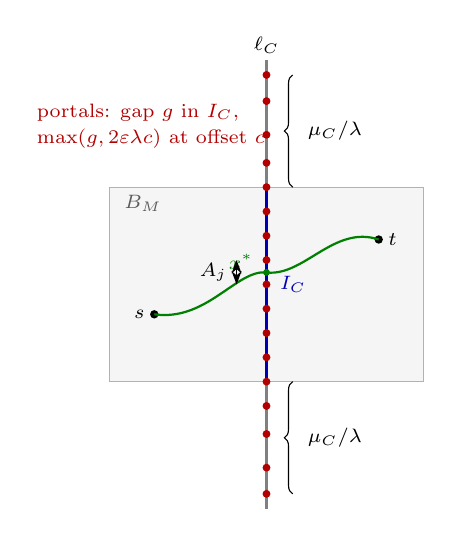
\begin{tikzpicture}[scale=0.95,>=Stealth]

  \draw[fill=gray!8,draw=gray!60] (0,0) rectangle (4.2,2.6);
  \node[gray!70!black,font=\scriptsize] at (0.45,2.38) {$B_M$};

  \draw[thick,gray] (2.1,-1.7) -- (2.1,4.3);
  \node[font=\scriptsize] at (2.1,4.5) {$\ell_C$};
  \draw[very thick,blue!70!black] (2.1,0) -- (2.1,2.6);
  \node[blue!70!black,font=\scriptsize,anchor=west] at (2.15,1.3) {$I_C$};

  \draw[decorate,decoration={brace,amplitude=3pt}] (2.45,2.6) -- (2.45,4.1)
    node[midway,right=2pt,font=\scriptsize] {$\mu_C/\lambda$};
  \draw[decorate,decoration={brace,amplitude=3pt,mirror}] (2.45,0) -- (2.45,-1.5)
    node[midway,right=2pt,font=\scriptsize] {$\mu_C/\lambda$};

  \foreach \y in {0,0.325,0.65,0.975,1.3,1.625,1.95,2.275,2.6} \fill[red!70!black] (2.1,\y) circle (1.5pt);

  \foreach \y in {2.925,3.3,3.75,4.1} \fill[red!70!black] (2.1,\y) circle (1.5pt);
  \foreach \y in {-0.325,-0.7,-1.15,-1.5} \fill[red!70!black] (2.1,\y) circle (1.5pt);

  \fill (0.6,0.9) circle (1.6pt) node[left,font=\scriptsize] {$s$};
  \fill (3.6,1.9) circle (1.6pt) node[right,font=\scriptsize] {$t$};
  \draw[thick,green!50!black] (0.6,0.9) .. controls (1.3,0.8) and (1.7,1.5) .. (2.1,1.46)
    .. controls (2.6,1.4) and (3.0,2.1) .. (3.6,1.9);
  \fill[green!50!black] (2.1,1.46) circle (1.3pt);
  \node[green!50!black,font=\scriptsize,anchor=east] at (2.05,1.6) {$x^\ast$};

  \draw[<->,font=\scriptsize] (1.7,1.3) -- (1.7,1.625) node[midway,left] {$A_j$};

  \node[red!70!black,font=\scriptsize,anchor=west] at (-1.1,3.6) {portals: gap $g$ in $I_C$,};
  \node[red!70!black,font=\scriptsize,anchor=west] at (-1.1,3.25) {$\max(g,2\eps\lambda c)$ at offset $c$};
\end{tikzpicture}
\caption{One cut of the index. The region $M$ has bounding box $B_M$, and the cut line $\ell_C$ meets it in
$I_C$. A shortest path from $s$ to $t$ must cross $\ell_C$ within the window, at most $\mu_C/\lambda$ from
$I_C$ (Lemma~\ref{lem:window}). Portals are placed at arc gap $g$ inside the box and at gaps growing with the
offset outside it. Both $s$ and $t$ store exact geodesic distances to all portals.}
\label{fig:cut}
\end{figure}

\subsection{Cut hierarchy and windows}

The index is built on a kd hierarchy of the vertices. A region $M$ is a set of vertices with chart bounding
box $B_M$. If the diagonal of $B_M$ is at most $R$, the region is a leaf. Otherwise we cut it along the axis
$a$ of the larger extent at a value $v$ strictly between the two middle member coordinates, chosen so that
no vertex of $T$ has $a$-coordinate $v$. The cut line is $\ell_C=\{x_a=v\}$, and the children are the
members on its two sides. We write $I_C=\ell_C\cap B_M$.

A shortest path between two members of $M$ on opposite sides of the cut must cross $\ell_C$ (by continuity of
its chart projection), but it may leave the box first. The window bounds how far. Pick a hub $h\in M$ near
the centre of the box and let $\mu_C = \max_{u\in M}\tilde U(h,u)$, where $\tilde U$ is the mesh-graph
distance, an upper bound of $d$ because a graph path is a curve on $T$.
\begin{lemma}[window]
\label{lem:window}
Let $s,t\in M$ lie on opposite sides of $\ell_C$, let $\gamma$ be a shortest path between them and
$x^\ast\in\gamma\cap\ell_C$. Then $d(s,t)\ge 2\lambda\,\dist(x^\ast,I_C)$, and $\dist(x^\ast,I_C)\le\mu_C/\lambda$.
\end{lemma}
\begin{proof}
By~\eqref{eq:lower}, $d(s,t)\ge\lambda(|s-x^\ast|+|x^\ast-t|)\ge 2\lambda\dist(x^\ast,B_M)$, and for a point
of $\ell_C$ the nearest point of $B_M$ lies on $I_C$. On the other side, $d(s,t)\le d(s,h)+d(h,t)\le 2\mu_C$.
\end{proof}
The window $W_C=\{x\in\ell_C:\dist(x,I_C)\le\mu_C/\lambda\}$ therefore contains every crossing that matters.
Its intersection with the surface is a union of segments, the runs, which we compute exactly from the faces
the line crosses. On each run the lifted cut is a polyline, and we measure arc length $A(\cdot,\cdot)$ along it.

\subsection{Portals and labels}

The portals $P_C$ of a cut are points of the runs, sorted along the line, including the ends of every run and
of $I_C$. For two consecutive portals of a run with arc distance $A_j$ we require
\begin{equation}
A_j \le g \text{ if the interval lies in } I_C, \qquad A_j\le\max(g,\,2\eps\lambda c_j)\text{ otherwise},
\label{eq:gaps}
\end{equation}
where $c_j$ is the chart distance from the interval to $I_C$. Inside the box the portals are dense; outside
it the gap grows linearly with the offset, which Lemma~\ref{lem:window} allows because a path crossing at
offset $c$ is at least $2\lambda c$ long. The tails therefore hold only $O(\eps^{-1}\log(\mu_C/\lambda R))$
portals.

Every member $u$ of $M$ stores the exact distances $\ell(u,p)=d(u,p)$ to all portals $p\in P_C$, and the
rows of all cuts on the path from $u$'s leaf to the root form its label. In addition, every vertex stores a
near table with the exact distances to all vertices within chart distance $R$.

\paragraph{Exact labels on small sub-meshes.}
A label is a geodesic distance on the whole surface, but it can be computed on a small part of it.
\begin{lemma}[ellipse]
\label{lem:ellipse}
If $d(x,u)\le D$, every point of a shortest path from $x$ to $u$ lies within chart distance $D/(2\lambda)$ of
the segment $[x,u]$.
\end{lemma}
\begin{proof}
By~\eqref{eq:lower}, a point $z$ of the path has $|z-x|+|z-u|\le D/\lambda$, so it lies in the ellipse with foci
$x,u$ and major axis $D/\lambda$, whose points are within its semi-minor axis
$\frac12\sqrt{(D/\lambda)^2-|x-u|^2}\le D/(2\lambda)$ of the segment.
\end{proof}
With $D$ a graph upper bound through the hub, all label geodesics of a cut stay inside the bounding box of
$M\cup P_C$ dilated by $D/(2\lambda)$. We take the faces that meet this box, insert the portals as vertices
(on their faces' planes, so the surface does not change), and run one exact single-source sweep per portal
on this sub-mesh. A geodesic of $T$ inside the sub-mesh is a curve of the sub-mesh and conversely, so the
sub-mesh distances are exact. The near tables are computed the same way, from one sweep per vertex on its
own small sub-mesh.

\subsection{Query and certificate}

\begin{algorithm}[t]
\caption{Query $(s,t)$}
\label{alg:query}
\begin{algorithmic}[1]
\If{$|s-t|\le R$} \Return $d(s,t)$ from the near table of $s$ \EndIf
\State $C\gets$ the deepest cut whose region contains $s$ and $t$
\State $f_j\gets\ell(s,p_j)+\ell(t,p_j)$ for every portal $p_j\in P_C$
\State $\UB\gets\min_j f_j$
\State $\LB\gets\max\big(\lambda|S-T|,\ \min_j[\tfrac12(f_j+f_{j+1})-A_j]\big)$ \Comment{consecutive portals of a run}
\State $\hat d\gets$ the interpolated minimum of $f$, clamped into $[\LB,\UB]$
\State \Return $(\hat d,\LB,\UB)$
\end{algorithmic}
\end{algorithm}

Algorithm~\ref{alg:query} answers a query. If $s$ and $t$ are not near, they lie in different leaves, hence on
opposite sides of the deepest cut $C$ whose region contains both. Every $f_j$ is the length of a path through
$p_j$, so $\UB=\min_j f_j\ge d(s,t)$. The lower bound uses that a label row is 1-Lipschitz along the cut in
arc length: $|\ell(u,p)-\ell(u,q)|\le A(p,q)$.

\begin{lemma}[sandwich]
\label{lem:sandwich}
$\LB\le d(s,t)\le\UB$ for every pair.
\end{lemma}
\begin{proof}
Near pairs are exact. Otherwise let $x^\ast$ be a crossing of a shortest path, which lies on a run between
consecutive portals $p_j,p_{j+1}$ by Lemma~\ref{lem:window}, and let $a=A(p_j,x^\ast)$. The cut itself is a
curve, so $d(x^\ast,p_j)\le a$, and
$f_j\le d(s,x^\ast)+a+a+d(x^\ast,t)=d(s,t)+2a$. Likewise $f_{j+1}\le d(s,t)+2(A_j-a)$. Adding gives
$\frac12(f_j+f_{j+1})-A_j\le d(s,t)$, and the chord term is a lower bound by~\eqref{eq:lower}.
\end{proof}

\begin{theorem}
\label{thm:main}
For every pair of vertices,
$(1-\eps)\,d(s,t)\le\LB\le d(s,t)\le\UB\le(1+\eps)\,d(s,t)$,
with equality when $|s-t|\le R$.
\end{theorem}
\begin{proof}[Proof sketch]
For a non-near pair, $d:=d(s,t)\ge\lambda|s-t|>\lambda R=g/\eps$ by~\eqref{eq:lower}. From the proof of
Lemma~\ref{lem:sandwich}, $\UB\le\min(f_j,f_{j+1})\le d+A_j$. If the crossing interval lies in $I_C$,
$A_j\le g<\eps d$. Otherwise its offset satisfies $d\ge 2\lambda c_j$ by Lemma~\ref{lem:window}, and
\eqref{eq:gaps} gives $A_j\le\max(g,2\eps\lambda c_j)\le\eps d$. The lower bound follows the same way: an
interval term is at least $d-A_j$, and a tail interval with $A_j>\eps d$ has both portals at offset more than
$d/(2\lambda)$, where every $f$ is at least $2\lambda c_j>d$. The full proof is in Appendix~\ref{app:proofs}.
\end{proof}

The certificate is not only a worst-case statement. $\UB/\LB$ is known for every answer, and it is usually
far below $1+\eps$: the median interval width is 0.7--2\% for vertex pairs in our experiments. The returned estimate is the
interpolated minimum of the label sum, which in our experiments is 3--4 orders of magnitude more accurate
than $\eps$.

\subsection{Capped portals and certify-or-refine}
\label{sec:capped}

The top cuts are long and have $\Theta(\sqrt n)$ portals each, and every vertex stores them, so the labels
grow like $n^{1.5}$ in total. The capped variant puts at most $k$ portals inside the box of each cut: its gap
is $g_C=\max(g,A(I_C)/k)$, and its tails step by $\max(g_C,2\eps\lambda c)$. Lemma~\ref{lem:sandwich} does not
use the gap, so the interval stays sound. Theorem~\ref{thm:main} needs $g_C\le\eps d$, which fails only for
pairs closer than $g_C/\eps$ across a capped cut. For these the query computes the distance exactly, with one
sweep on the faces meeting $\mathrm{bbox}(s,t)$ dilated by $\UB/(2\lambda)$ (Lemma~\ref{lem:ellipse}).
\begin{theorem}
\label{thm:capped}
In the capped index every answer satisfies $\UB\le(1+\eps)\LB$ or is exact. A cut has at most
$k+O(\eps^{-1}\log k)$ portals, so the labels hold $O\big((k+\eps^{-1}\log k)\,n\log n\big)$ entries.
\end{theorem}
The tail count follows from $g_C\approx\sigma A(I_C)/k$: a tail first steps by $g_C$ for $O(1/\eps)$ portals
and then grows geometrically up to the window, whose length is about $A(I_C)/\lambda$, which takes
$O(\eps^{-1}\log k)$ portals. A uniformly random pair needs the exact route with probability about
$2\pi/(k\eps)^3$, and we measured no refined pair at all among 1,500 pairs at 10k vertices and 200 at 100k.

\subsection{Arbitrary surface points}
\label{sec:a2a}

For a point $p$ on face $f$ with corners $a_i$ and a point $q$ on face $f'$ with corners $b_j$, the straight
segment inside a face is a path, so $d(p,a_i)\le w_f|P-A_i|$. The vertex certificates and the triangle
inequality give
\begin{align*}
\UB(p,q) &= \min_{i,j}\ w_f|P-A_i|+\UB(a_i,b_j)+w_{f'}|Q-B_j|,\\
\LB(p,q) &= \max\Big(\lambda|P-Q|,\ \max_{i,j}\ \LB(a_i,b_j)-w_f|P-A_i|-w_{f'}|Q-B_j|\Big).
\end{align*}
Pairs within $R$, and pairs whose interval is wider than $1+2\eps$, are computed exactly by one sweep between
the two points on an ellipse sub-mesh.
\begin{theorem}
\label{thm:a2a}
Every A2A answer satisfies $\LB\le d(p,q)\le\UB\le(1+2\eps)\LB$.
\end{theorem}

\subsection{Complexity}

\begin{table}[t]
\caption{Size, query and build of the two variants. $D$: side of the chart; $\bar\sigma$: mean metric speed
along the cuts; $\rho$: vertex density; $K_C$: portals of the answering cut. Build times assume a sweep over
$m$ faces costs $O(m\log m)$.}
\label{tab:complexity}
\small
\begin{tabular}{@{}lll@{}}
\toprule
& kd (Theorem~\ref{thm:main}) & capped (Theorem~\ref{thm:capped})\\
\midrule
labels & $\Theta(n^{1.5})$; $\approx 3\bar\sigma D/g$ per vertex & $O((k+\eps^{-1}\log k)\,n\log n)$\\
near tables & $\pi\rho g^2/(\eps\lambda)^2$ per vertex & same\\
query & $O(\text{depth}+K_C)$ & same, plus a rare exact sweep\\
build & $\Theta(n^{1.5}\log n)$ & $O((k+\eps^{-1}\log k)\,n\log^2 n)$\\
\bottomrule
\end{tabular}
\end{table}

Table~\ref{tab:complexity} summarises the costs. A cut at level $\ell$ of the hierarchy sweeps sub-meshes of
$\Theta(n/2^\ell)$ faces, one per portal, and there are $O(\log n)$ levels. Uncapped, the top cuts dominate:
$\Theta(\sqrt n)$ portals each over $\Theta(n)$ faces. The cap bounds the number of sweeps per cut by the
number of portals, so the capped build is near-linear as well. The near tables add $O(n\eps^{-2}\log n)$ to
both. We state plainly that the asymptotic space of Djidjev and Sommer~\cite{djidjev2011approximate} is
smaller than that of our uncapped index; our contribution is an implemented index that certifies every
answer, with constants we measure.

\section{Engineering}
\label{sec:engineering}

\paragraph{Hybrid exact sweeps.}
We use two exact solvers: Kirsanov's implementation of MMP~\cite{surazhsky2005fast} and
VTP~\cite{qin2016fast}. VTP is 2.6--4.1 times faster per full sweep, but its vertex queue does not make a
popped vertex final, so it has no exact early stop. MMP processes windows in order of their minimum
distance, and once that minimum exceeds the current value at every target no later window can improve any of
them, so it stops early without changing a single distance. For each cut we choose MMP when the sub-mesh is
large relative to the members' box, and VTP otherwise. VTP needs its per-sweep state reset and consistently
oriented faces; it links its window lists from the first edge, so it also rejects sub-meshes that fall into
several pieces, which we sweep piece by piece. On Gunnison10k the hybrid build takes 202\,s, against 284\,s
with MMP alone and 215\,s with VTP alone, with identical labels.

\paragraph{Closed-loop label coding.}
Labels are stored as float32 by default, rounded up so that they stay upper bounds bit-exactly, and lower
bounds subtract the matching relative margin. Most of the index is label rows, and neighbouring entries of a
row differ by at most the arc gap between their portals (the rows are 1-Lipschitz). We therefore code a row in
runs of deltas with 16 or 8 bits, anchored by a float32 value per run, and encode in a closed loop: each code
is chosen from the decoded value of the previous entry, so the error does not accumulate. Every decoded value
is at least the stored one, so the upper bound stays an upper bound; the lower bound subtracts the bounded
decoding error, and the estimate is de-biased by half of it. A block scan over 8 portals at a time with four
accumulators keeps the decoding cost low. The near tables are stored once per pair, in the row of the smaller
vertex id, with varint id deltas; ratio-coded variants with 16 and 8 bits store
$D=|PQ|(1+c\,q)$ with the least code $c$ that is not below the true distance.

\paragraph{Parallel build.}
The top cuts spread their portals over the threads and the remaining cuts go one per thread. The labels are
bit-identical to a single-threaded build, two threads give a $2.0\times$ speed-up, and the peak memory is
about the coded index size because rows are coded as soon as a cut is done. A memory gate bounds the solvers
alive at once. All timings in this paper use one thread.

\paragraph{Certified proximity queries.}
For a kNN or range query from $s$ over a set of objects, the index gives an interval for each candidate. An
object whose $\UB$ is below the $k$-th smallest $\LB$ is in the answer, one whose $\LB$ exceeds the $k$-th
smallest $\UB$ is not, and only the ambiguous ones need an exact sweep from $s$, which we run once for all of
them on an ellipse sub-mesh. Without that sweep, returning the $k$ objects of smallest $\UB$ is a certified
$\eps$-approximate kNN: every returned object has $d\le(1+\eps)d_k$, with $d_k$ the true $k$-th distance.
Likewise, the objects with $\UB\le r$ form a range answer with no false positives that contains every object
within $r/(1+\eps)$.

\paragraph{Weighted terrains.}
Exact weighted geodesics have no practical algorithm, so on weighted terrains the labels are distances in a
Steiner graph with $m$ points per edge, shared by all searches and searched with a stop once all members of a
cut are settled. Graph paths are curves on the surface, so $\UB$ is still the cost of an actual path, but the
labels are not exact, so the interval lower bound no longer holds and we keep only the chord bound
$\lambda|S-T|$. The weighted index therefore returns an upper bound and an estimate, not a $(1+\eps)$
certificate.

\paragraph{Obstacles.}
An obstacle removes the faces whose chart centroid lies inside it, so the surface gets a hole and paths go
around it. The certificate needs no change. A hole only lengthens paths, so every chart lower bound still
holds; $\mu_C$ is a graph distance on the holed mesh, so a detour widens the window by itself; a cut line
broken by holes gives several runs, each bracketed by portals at its ends; and the near tables hold every pair
within chart radius $R$ with its exact distance, including pairs close in the chart but separated by a wall.
One practical point matters. Where two holes touch at a single vertex the mesh is no longer a manifold, and
there Kirsanov's MMP returned distances up to 5\% too long, longer than a path in a Steiner graph. We
therefore separate touching holes by keeping the largest fan of faces at such vertices; on the cleaned pilot
meshes MMP and VTP agree to $10^{-15}$. On the larger meshes VTP in turn returns slightly too long
distances at a few vertices (Section~\ref{sec:server}), so the ground truth is MMP.

\section{Experiments}
\label{sec:experiments}

\paragraph{Setup.}
The experiments on the small terrains run on an Apple M1 laptop (8\,GB), and those on terrains with
0.5--2.5M faces on an HPC cluster (Section~\ref{sec:server}); every method runs on one thread. Our index is
implemented in C++17. The ground truth is exact MMP in double precision. We use the four benchmark terrains of the
SE-Oracle and EAR-Oracle papers (HorseMount, BigMount, HeadlightMount, RobinsonMountain, 793--3,696
vertices), Gunnison10k (9,610 vertices) and a 100k-vertex DEM, GunnisonForest100k. Our index and DGG answer the
same 1,500 random vertex pairs per terrain (seed 7). EAR-Oracle and the other methods of its authors' harness
answer 100 pairs with the points moved 5\,cm into a face, because the harness cannot locate a point exactly at a
vertex. The portal gap $g$ is given in mean edge lengths, and we report $\eps$ and $g$ per experiment.

\paragraph{Competitors.}
Every competitor runs with its authors' code: SE-Oracle, EAR-Oracle, K-Algo and the on-the-fly Steiner
schemes in the harness of the EAR-Oracle authors~\cite{huang2023ear}, with a fix for weighted endpoints that
changes their published weighted errors; UP-Oracle, WSPD-Oracle and RC-Oracle from the UP-Oracle
code~\cite{yan2025up}; DGG~\cite{adikusuma2020fast} with a port to our platform; NeuroGF~\cite{zhang2023neurogf}
with the authors' network and training, trained on exact distances and paths of our terrains; and exact MMP and
VTP on the fly.

\subsection{Main comparison}

\begin{table*}[t]
\caption{Vertex-to-vertex queries, one thread. Ours: $\eps=0.1$, $g=0.5$ edges, hybrid sweeps, float32 labels.
Columns: build time / index size / query time / mean error / maximum error. Every answer of ours is certified
and correct ($\LB\le d\le\UB$ on all pairs); none of the other methods returns a bound.}
\label{tab:main}
\small
\begin{tabular}{@{}lrllll@{}}
\toprule
terrain & $n$ & ours & EAR-Oracle (sp 5) & DGG ($\eps=10^{-4}$) & VTP\\
\midrule
HorseMount & 793 & 3.1\,s / 1.3\,MB / 0.18\,$\mu$s / 0.024\% / 1.16\% & 23.5\,s / 189\,MB / 1.3\,ms / 3.10\% / 24.5\% & 0.73\,s / 4.4\,MB / 1.4\,ms / 0.0023\% / 0.02\% & 3.3\,ms\\
BigMount & 1,440 & 10.4\,s / 3.3\,MB / 0.23\,$\mu$s / 0.022\% / 0.86\% & 52.4\,s / 319\,MB / 1.8\,ms / 3.19\% / 6.41\% & 1.5\,s / 8.9\,MB / 2.6\,ms / 0.0025\% / 0.02\% & 6.6\,ms\\
HeadlightMount & 2,470 & 29.1\,s / 6.5\,MB / 0.25\,$\mu$s / 0.016\% / 1.30\% & 107\,s / 592\,MB / 2.5\,ms / 3.29\% / 8.47\% & 2.9\,s / 16.8\,MB / 5.5\,ms / 0.0026\% / 0.02\% & 12.0\,ms\\
RobinsonMountain & 3,696 & 44.1\,s / 10.7\,MB / 0.28\,$\mu$s / 0.020\% / 1.79\% & 188\,s / 672\,MB / 3.8\,ms / 3.50\% / 8.60\% & 4.5\,s / 25.3\,MB / 7.9\,ms / 0.0023\% / 0.02\% & 18.1\,ms\\
Gunnison10k & 9,610 & 202\,s / 37.4\,MB / 0.36\,$\mu$s / 0.0076\% / 0.37\% & 672\,s / 702\,MB / 10.2\,ms / 3.43\% / 9.37\% & 13.2\,s / 72.8\,MB / 22.3\,ms / 0.0028\% / 0.01\% & 55.0\,ms\\
\bottomrule
\end{tabular}
\end{table*}

\begin{figure*}[t]
\centering
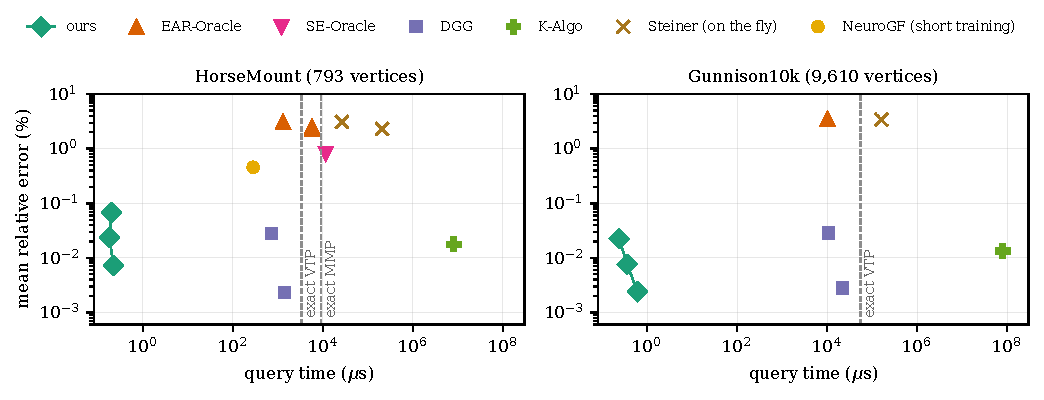
\includegraphics[width=0.9\textwidth]{figures/fig_methods.pdf}
\caption{Query time against mean error for every method we ran, on the smallest benchmark terrain and on
Gunnison10k. The three points of ours are $\eps=0.05,0.1,0.2$. Dashed lines mark the exact solvers, which have
no error. NeuroGF was trained with a short budget on HorseMount only; its full-budget runs at 0.5M faces are in
Section~\ref{sec:server}.}
\label{fig:methods}
\end{figure*}

Table~\ref{tab:main} and Figure~\ref{fig:methods} compare the methods.

\paragraph{Query time.}
\cci answers in 0.18--0.36\,$\mu$s. EAR-Oracle takes 1.3--10.2\,ms, so we are 7,000--28,000 times faster, and
DGG, which runs Dijkstra on its graph, takes 1.4--22\,ms. An exact VTP sweep per query costs 3.3--55\,ms, and
K-Algo and the on-the-fly Steiner schemes are slower still (Figure~\ref{fig:methods}).

\paragraph{Accuracy.}
With $\eps=0.1$ our mean error is 0.0076--0.024\% and the maximum 0.37--1.79\%, while EAR-Oracle has a mean
error of 3.1--3.5\% and a maximum of 6.4--24.5\%. Its nominal $\eps$ is relative to its Steiner graph, and the
Steiner graph with 5 points per edge is itself about 3\% longer than the surface. Increasing the number of
Steiner points to 10 and 20 on HorseMount lowers EAR-Oracle's mean error only to 2.5\% and 2.3\%, at 541 and
683\,MB. SE-Oracle reaches 0.81\% after 1.7\,h of build and 942\,MB on HorseMount. DGG is the most accurate
approximate method, with mean errors of about 0.0025\%, but its queries are four orders of magnitude slower
than ours and return no bound.

\paragraph{Certificates.}
All 7,500 answers in Table~\ref{tab:main} are certified and correct. The guaranteed bound is never violated,
and it is about two times conservative in the worst case: with $\eps=0.1$ the largest $\UB$ error over all
pairs is 0.9--3.4\%, against the guaranteed 10\%.

\paragraph{Size and build.}
The index is 1.3--37\,MB, 19--145 times smaller than EAR-Oracle's, and builds 3--8 times faster.
DGG's graph is two to three times larger than our index and builds faster.

\subsection{Size against error}

\begin{figure*}[t]
\centering
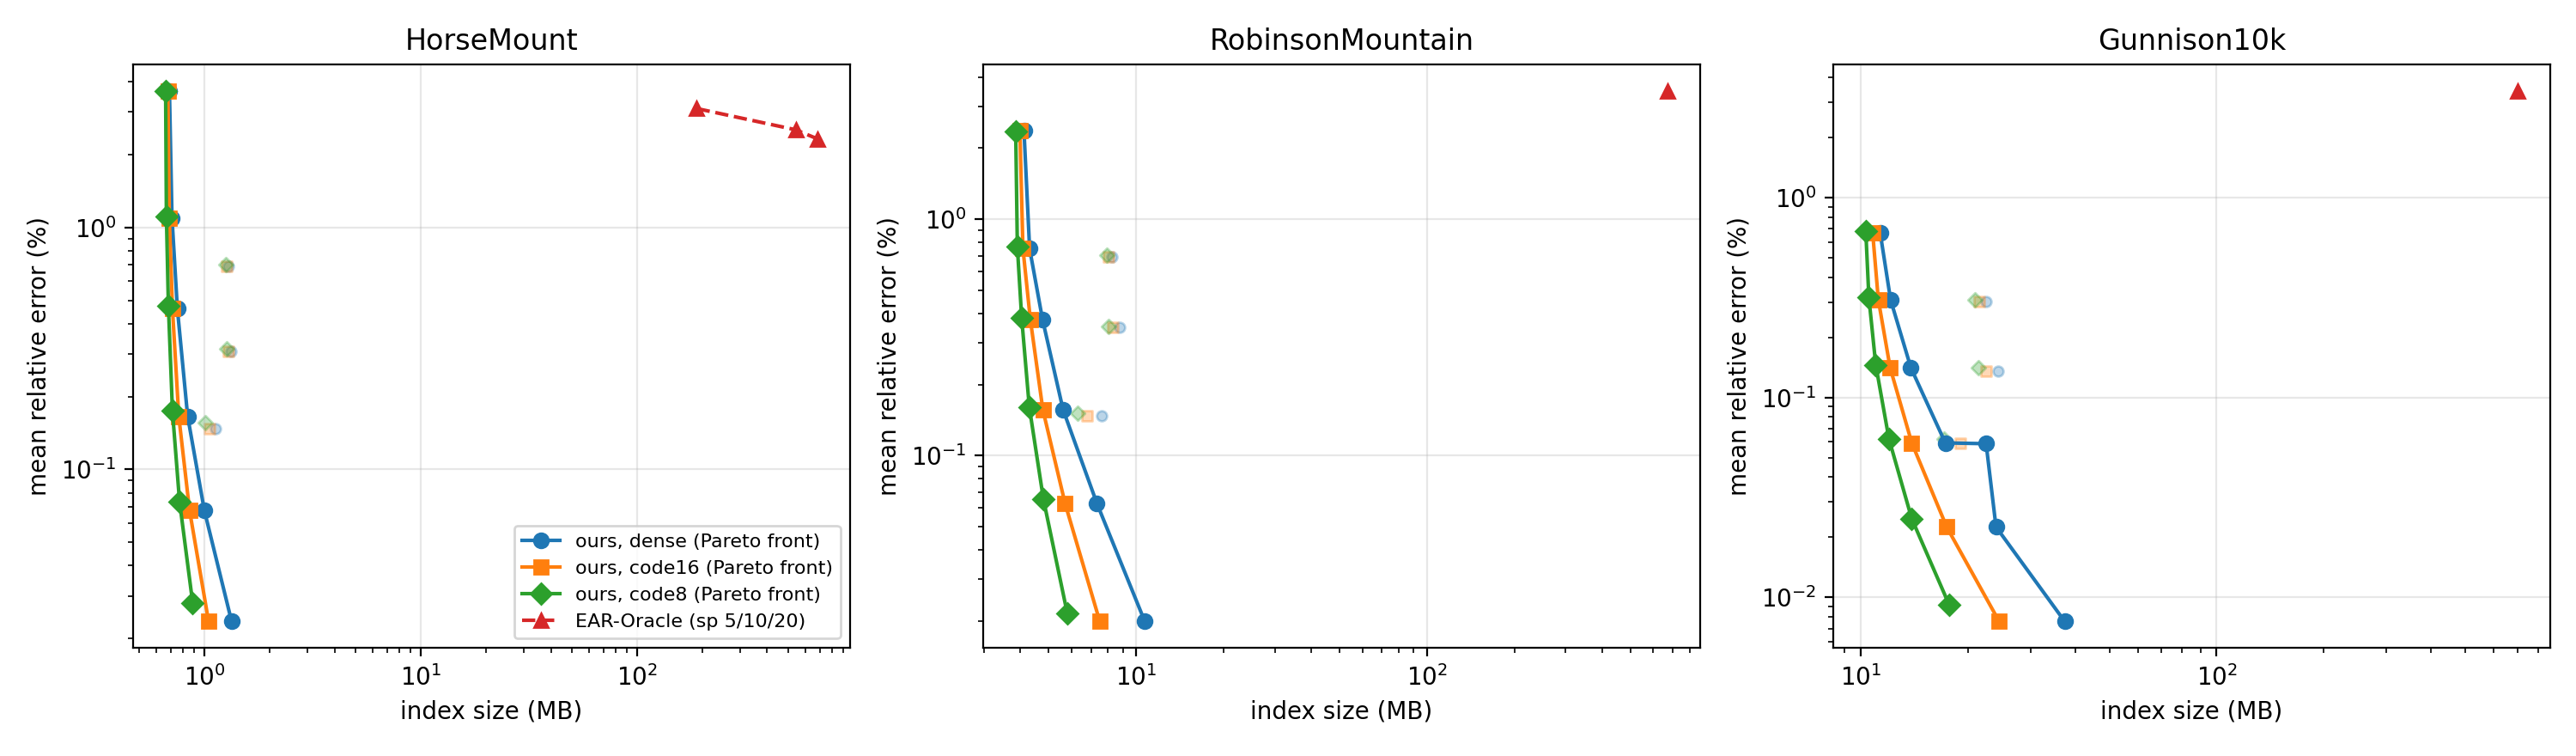
\includegraphics[width=0.95\textwidth]{figures/fig_size_error.png}
\caption{Index size against mean error. Each curve is the Pareto front of our index over $\eps$ and $g$ for one
label storage (float32, 16-bit and 8-bit codes); faded points are dominated settings. Triangles are EAR-Oracle
with 5, 10 and 20 Steiner points per edge.}
\label{fig:size}
\end{figure*}

Figure~\ref{fig:size} shows the size against the mean error over a sweep of $\eps$ and $g$. Our fronts lie
entirely below and to the left of EAR-Oracle: on Gunnison10k the coarsest setting, $\eps=1$ at 21\,MB, has a
mean error of 0.31\%, ten times lower than EAR-Oracle's best, at a 30th of its size. Pushing $\eps$ up to 3.2
with a fixed near radius brings our error to EAR-Oracle's level: 3.7\% at 0.66\,MB on HorseMount against
EAR-Oracle's 3.1\% at 189\,MB, and 2.4\% at 3.9\,MB on RobinsonMountain against 3.5\% at 672\,MB. Every answer
stays certified. On Gunnison10k, $\eps=0.05,0.1,0.2$ give 64, 37 and 24\,MB with mean errors of 0.0024\%,
0.0076\% and 0.023\%.

\paragraph{100k vertices.}
Table~\ref{tab:storage} gives the storage variants on GunnisonForest100k with $\eps=0.2$. The float32 index takes
534\,MB, the 8-bit codes reduce it to 224\,MB with the mean error going from 0.0069\% to 0.0075\%, and a cap of 50
portals per cut brings it to 177\,MB at 0.041\%. No pair needed refining. EAR-Oracle did not finish on this
terrain on the 8\,GB laptop; on the cluster it needs 93\,GB and 5.4\,h (Section~\ref{sec:server}). $\eps_c$-covers in the style of
Thorup~\cite{thorup2004compact}, which keep for every vertex only the portals needed to reach the rest of the cut,
are dominated by the 8-bit codes at every size we tried: at 100k, covers with $\eps_c=0.05$ take 230\,MB for a mean
error of 0.79\%. The shifted hierarchy, three shifted quadtrees with a gap that grows with the cell size,
is 1.4 times larger than the kd hierarchy at 100k vertices, as its constants predict; it becomes smaller from 1M
faces (Section~\ref{sec:server}).

\begin{table}[t]
\caption{Storage variants on GunnisonForest100k (100,511 vertices), $\eps=0.2$, one thread.}
\label{tab:storage}
\small
\begin{tabular}{@{}llrrr@{}}
\toprule
hierarchy & labels & size & mean error & query\\
\midrule
kd & float32 & 534\,MB & 0.0069\% & 0.38\,$\mu$s\\
kd & 16-bit & 330\,MB & 0.0069\% & --\\
kd & 8-bit & 224\,MB & 0.0075\% & 1.3\,$\mu$s\\
cap 100 & 8-bit & 198\,MB & 0.017\% & --\\
cap 50 & float32 & 346\,MB & 0.039\% & --\\
cap 50 & 8-bit & 177\,MB & 0.041\% & 0.64\,$\mu$s\\
kd & covers $\eps_c=0.05$ & 230\,MB & 0.79\% & --\\
\bottomrule
\end{tabular}
\end{table}

\paragraph{Growth with $n$.}
From 0.8k to 100k vertices the build time grows like $n^{1.45}$ and the index like $n^{1.32}$, close to the
$n^{1.5}$ of Table~\ref{tab:complexity}; the 100k build takes 41--66\,min on the laptop, depending on the load.
The capped variant and the larger terrains are the subject of Section~\ref{sec:server}.

\subsection{Arbitrary points}

\begin{table}[t]
\caption{Certified A2A queries, $\eps=0.1$, 100 random pairs of surface points per terrain.}
\label{tab:a2a}
\small
\begin{tabular}{@{}lrrrr@{}}
\toprule
terrain & query & mean err. & max err. & max $\UB$ err.\\
\midrule
HorseMount & 123\,$\mu$s & 0.11\% & 0.63\% & 6.2\%\\
BigMount & 111\,$\mu$s & 0.14\% & 2.69\% & 20.2\% (10.2\%)\\
HeadlightMount & 89\,$\mu$s & 0.076\% & 0.77\% & 5.9\%\\
RobinsonMountain & 85\,$\mu$s & 0.11\% & 0.97\% & 11.4\%\\
Gunnison10k & 78\,$\mu$s & 0.034\% & 0.23\% & 3.3\%\\
\bottomrule
\end{tabular}
\end{table}

Table~\ref{tab:a2a} gives the certified A2A queries. Every answer is sound, the mean error is 0.03--0.14\%,
and a query takes 78--123\,$\mu$s, because the four corner pairs are looked up and a few pairs are refined. The
refine step bounds the worst case: on BigMount one pair in 100 was refined, and the largest $\UB$ error fell from
20.2\% to 10.2\%. On the same kind of queries EAR-Oracle has a mean error of 4.9\% and a maximum of 87\% on
HorseMount, at 4.4\,ms per query.

\subsection{Weighted terrains}

On HorseMount with the face weights of the EAR-Oracle benchmark, our index with a Steiner graph of 5 points per
edge has a mean error of 0.35\%, a build time of 10.9\,s, a size of 2.9\,MB and a query time of 1.3\,$\mu$s,
measured against the shortest path found by any method. EAR-Oracle with 5 Steiner points has 2.42\% at 25.9\,s,
166\,MB and 1.14\,ms. Against a Steiner graph with 24 points per edge as the reference, our C++ index has a mean
error of 0.38\% with 5 points per edge and 0.23\% with 10.

\subsection{Obstacles}

\begin{figure}[t]
\centering
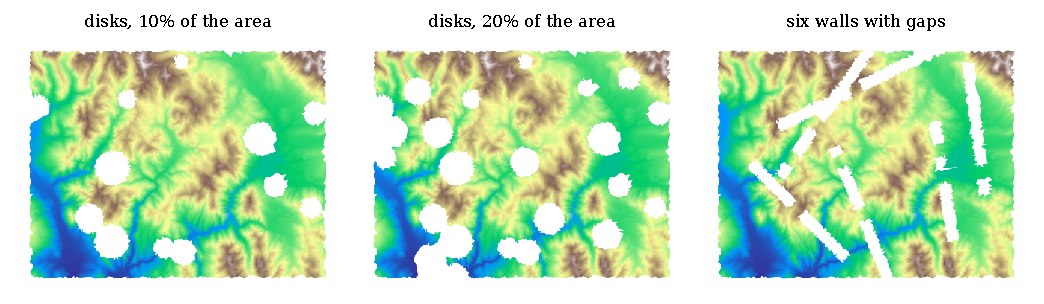
\includegraphics[width=\columnwidth]{figures/fig_obstacles.pdf}
\caption{The obstacle meshes of the pilot on Gunnison10k. The faces inside the obstacles are removed.}
\label{fig:obstacles}
\end{figure}

\begin{table}[t]
\caption{Obstacles on Gunnison10k (Figure~\ref{fig:obstacles}), ours with $\eps=0.2$, $g=1$ edge, cap 64. The
last column counts the random pairs whose distance is at least 1.2 times their straight-line distance.}
\label{tab:obstacles}
\small
\begin{tabular}{@{}lrrrrr@{}}
\toprule
obstacles & build & mean err. & max $\UB$ err. & sound & pairs $\ge 1.2$\\
\midrule
disks, 10\% & 61\,s & 0.033\% & 4.3\% & yes & 5\\
disks, 20\% & 55\,s & 0.044\% & 1.1\% & yes & 20\\
six walls & 131\,s & 0.032\% & 2.2\% & yes & 208\\
\bottomrule
\end{tabular}
\end{table}

Table~\ref{tab:obstacles} gives a pilot on Gunnison10k with the obstacles of Figure~\ref{fig:obstacles}. Every
answer is certified and correct, uncapped and capped, over random, near, distance-band and A2A pairs, including
the 208 pairs whose shortest path on the walls mesh is at least 20\% longer than the straight line. The mean error
is 0.03--0.04\%, as without obstacles. On the walls mesh EAR-Oracle has a mean error of 3.59\% and a maximum of
7.26\%, with 36\,ms per query and an index of 173\,MB, and DGG ($\eps=10^{-3}$) has a mean error of 0.027\% at
8.4\,ms per query.

\subsection{Proximity queries}

On HorseMount, a certified kNN query with $k=50$ over all vertices takes 27\,$\mu$s in the approximate mode, against
0.5\,ms for the exact answer from the index with refine and 0.85\,ms for an on-the-fly search pruned by chart
distances. On Gunnison10k with random objects the approximate mode answers kNN in 5\,$\mu$s for $k=1$,
20\,$\mu$s for $k=10$ and 165\,$\mu$s for $k=100$, and range queries in 2--7\,$\mu$s. In all our runs its recall
against the exact answer was at least 99.2\%, and the guarantees of Section~\ref{sec:engineering} held on every
query. The exact mode
needs one sweep only for the objects near the boundary of the answer; at 100k vertices it is 60 times faster than
the pruned on-the-fly search for $k=1$ and 1--2 times faster for large $k$, where that sweep dominates.

\subsection{The POI setting}

UP-Oracle and its baselines answer queries between a fixed set of points of interest. In that setting the simplest
exact index is a $P\times P$ table built by one VTP sweep per POI. It is exact, sub-microsecond, and the cheapest
to build for up to about 1,000 POIs on our terrains, which neither UP-Oracle nor our index beats. Our index in POI
mode, which indexes only the POIs, becomes smaller than the table from about 1,000 POIs, and at 3,000 POIs on
Gunnison10k it takes 3.1\,MB against the table's 36\,MB. Our index is designed for queries between all vertices and
arbitrary points, where no table fits.

\subsection{Terrains with 0.5--2.5M faces}
\label{sec:server}

The rest of the evaluation runs on the six terrains of the UP-Oracle paper~\cite{yan2025up} (TJ, SC, VS, AU, GI,
LH) at 0.5M, 1M, 1.5M, 2M and 2.5M faces, on an HPC cluster node with two Intel Xeon Gold 6248R processors and
768\,GB of memory. Every method runs on one thread, except NeuroGF, which trains and is queried on one V100 GPU
(we also report its single-thread CPU query time). The ground truth is exact MMP in double precision. Each terrain
has 2,000 random vertex pairs (200 sources with 10 targets), 2,000 pairs closer than the near radius, 300 pairs in
each of up to ten distance bands, and 200 pairs of arbitrary surface points; all methods answer the same pairs. Ours
uses $\eps=0.2$ and $g=1$ edge unless stated, so its index is smaller than in Table~\ref{tab:main}. Over all runs of
our index on the cluster, 5.46 million answers were checked against the ground truth, over every query set and
storage variant, and every one was certified and correct.

\begin{table*}[t]
\caption{Our index on the six terrains at 0.5M faces (251,001 vertices), $\eps=0.2$, $g=1$, one thread. Errors are
over the 2,000 random vertex pairs; the maximum $\UB$ error is the largest $(\UB-d)/d$. Uncapped: float32 / 8-bit
size, errors and query time of float32 labels. Cap 64: 8-bit labels. Every answer is certified and correct.}
\label{tab:server-ours}
\small
\begin{tabular}{@{}l|rrrrr|rrrrr|rr@{}}
\toprule
 & \multicolumn{5}{c|}{uncapped} & \multicolumn{5}{c|}{cap 64} & \multicolumn{2}{c}{NeuroGF}\\
terrain & build & size & query & mean err. & max err. & build & size & query & mean err. & max err. & mean & max\\
\midrule
TJ & 11.5\,h & 1.99 / 1.02\,GB & 1.43\,$\mu$s & 0.0012\% & 0.27\% & 7.3\,h & 358\,MB & 0.55\,$\mu$s & 0.021\% & 1.16\% & 0.40\% & 13.4\%\\
SC & 11.5\,h & 1.98 / 0.61\,GB & 1.47\,$\mu$s & 0.0011\% & 0.21\% & 7.5\,h & 357\,MB & 1.15\,$\mu$s & 0.021\% & 1.72\% & 0.39\% & 6.5\%\\
VS & 13.7\,h & 2.14 / 0.66\,GB & 1.39\,$\mu$s & 0.0012\% & 0.19\% & 8.6\,h & 366\,MB & 0.64\,$\mu$s & 0.029\% & 3.15\% & 0.56\% & 11.6\%\\
AU & 9.2\,h & 1.93 / 0.91\,GB & 0.91\,$\mu$s & 0.0011\% & 0.15\% & 6.0\,h & 355\,MB & 0.53\,$\mu$s & 0.014\% & 0.67\% & 0.21\% & 4.1\%\\
GI & 9.6\,h & 2.02 / 0.62\,GB & 1.47\,$\mu$s & 0.0016\% & 0.21\% & 6.2\,h & 359\,MB & 0.53\,$\mu$s & 0.029\% & 4.52\% & 0.44\% & 11.4\%\\
LH & 9.8\,h & 1.95 / 1.05\,GB & 1.41\,$\mu$s & 0.0015\% & 0.30\% & 7.2\,h & 356\,MB & 1.05\,$\mu$s & 0.020\% & 1.84\% & 0.34\% & 9.0\%\\
\bottomrule
\end{tabular}
\end{table*}

\begin{table}[t]
\caption{All methods on TJ and GI at 0.5M faces, vertex pairs, one CPU thread. Ours with 8-bit labels. NeuroGF
trains on a V100 GPU; its query time is on one CPU thread (0.3--0.4\,$\mu$s batched on the GPU). Only ours returns
a certified bound.}
\label{tab:server-comp}
\small
\setlength{\tabcolsep}{3pt}
\begin{tabular}{@{}llrrrrr@{}}
\toprule
 & method & build & size & query & mean & max\\
\midrule
\multirow{9}{*}{TJ} & ours, uncapped & 11.5\,h & 1.0\,GB & 1.7\,$\mu$s & 0.0017\% & 0.28\%\\
 & ours, cap 64 & 7.3\,h & 0.36\,GB & 0.55\,$\mu$s & 0.021\% & 1.16\%\\
 & ours, $\eps=0.1$ & 21.7\,h & 2.1\,GB & 2.6\,$\mu$s & 0.0006\% & 0.055\%\\
 & EAR-Oracle, sp 5 & 17.6\,h & 333\,GB & 426\,ms & 2.61\% & 9.75\%\\
 & EAR-Oracle, sp 7 & 35.4\,h & 468\,GB & 343\,ms & 1.91\% & 6.90\%\\
 & DGG, $10^{-3}$ & 2\,min & 0.76\,GB & 280\,ms & 0.035\% & 0.16\%\\
 & DGG, $10^{-4}$ & 7\,min & 2.4\,GB & 819\,ms & 0.0040\% & 0.036\%\\
 & NeuroGF (800 ep.) & 6.9\,h & 0.25\,MB & 0.39\,ms & 0.36\% & 9.1\%\\
 & exact VTP & -- & -- & 4.2\,s & 0 & 0\\
\midrule
\multirow{7}{*}{GI} & ours, uncapped & 9.6\,h & 0.62\,GB & 2.2\,$\mu$s & 0.0025\% & 0.21\%\\
 & ours, cap 64 & 6.2\,h & 0.36\,GB & 0.53\,$\mu$s & 0.029\% & 4.52\%\\
 & ours, $\eps=0.1$ & 18.9\,h & 1.3\,GB & 3.4\,$\mu$s & 0.0008\% & 0.077\%\\
 & EAR-Oracle, sp 5 & 21.3\,h & 333\,GB & 993\,ms & 2.85\% & 8.46\%\\
 & DGG, $10^{-4}$ & 7\,min & 2.4\,GB & 814\,ms & 0.0036\% & 0.015\%\\
 & NeuroGF & 3.5\,h & 0.25\,MB & 0.37\,ms & 0.44\% & 11.4\%\\
 & exact VTP & -- & -- & 3.9\,s & 0 & 0\\
\bottomrule
\end{tabular}
\end{table}

\begin{figure*}[t]
\centering
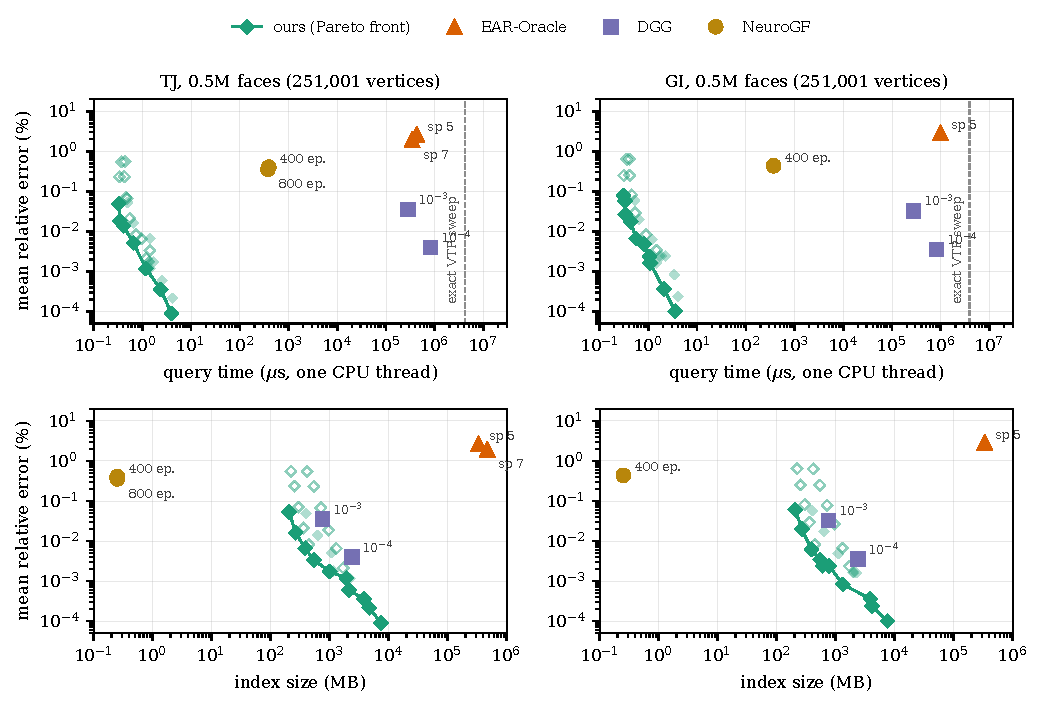
\includegraphics[width=0.92\textwidth]{figures/fig_server_methods.pdf}
\caption{Query time (top) and index size (bottom) against mean error on TJ and GI at 0.5M faces. Our points cover
the uncapped index, $\eps=0.1$, caps $k=8,\dots,256$ and a sweep of $\eps$ and $g$, each with float32 and 8-bit
labels; hollow points are capped and the line is the Pareto front.}
\label{fig:server-methods}
\end{figure*}

\paragraph{Main comparison at 0.5M faces.}
Tables~\ref{tab:server-ours} and~\ref{tab:server-comp} and Figure~\ref{fig:server-methods} give the results.
Uncapped, our index answers in 0.9--1.5\,$\mu$s with a mean error of 0.0011--0.0016\% and a maximum of 0.15--0.30\%,
in 1.9--2.1\,GB of float32 labels or 0.6--1.1\,GB of 8-bit codes, built in 9--14\,h on one thread. With a cap of
64 portals per cut it takes 355--366\,MB, answers in 0.5--1.2\,$\mu$s with a mean error of 0.014--0.029\%, and builds in
6--9\,h; on TJ and GI the exact refine was needed for one pair each. EAR-Oracle with its default of 5 Steiner points per edge needs
333\,GB and 17--21\,h, answers in 0.4--1.0\,s, and has a mean error of 2.6--2.9\% and a maximum of 8.5--9.8\%. With 7
points it needs 468\,GB and 35\,h and still has 1.9\%. Its peak memory follows from its design: every leaf box stores
the distances between its boundary vertices and all Steiner points inside it, both ways, in a balanced tree, which
grows like the number of Steiner points times $n^{1.5}$ for a fixed number of boxes. On the authors' own
GunnisonForest (100,511 vertices) it needs 93\,GB and 5.4\,h, with a mean error of 2.9\%; our index on the same
terrain takes 480\,MB, 1.0\,h and 0.0077\%. So our index is 330--930 times smaller, answers five to six orders of magnitude faster, and its mean error is
three orders of magnitude lower.

DGG is the strongest competitor in accuracy and build time: its graph builds in minutes, and with $\eps=10^{-4}$ its
mean error is 0.004\%, comparable to ours. But a DGG query is a Dijkstra search on a graph of 0.8--2.4\,GB and takes
0.28--0.82\,s, and it returns no bound. At the same size our index is more accurate: with $\eps=0.4$ and $g=1$ and
8-bit labels, 1.0\,GB on TJ gives 0.0017\% against DGG's 0.0040\% at 2.4\,GB (Figure~\ref{fig:server-methods}).
We see DGG and our index as answering different needs:
DGG is the better choice for a handful of queries on a terrain that will not be queried again, ours when the terrain is
queried many times, needs answers in microseconds, or needs a bound on each answer.
NeuroGF is the smallest index by far, 0.25\,MB of network weights, but its mean error is 0.2--0.6\% and single
pairs are off by 4--13\%, with no indication of which. We checked that this is not an artefact of our setup.
Distance-to-surface targets measured exactly instead of against a subsampled surface give the same accuracy (0.41\%
against 0.40\% on TJ), and 800 epochs instead of their 400 lower the mean error by 11--15\% and the maximum from 13.4\%
to 9.1\%, at twice the training time. An exact VTP sweep takes 3.9--4.2\,s per query.

\paragraph{When the build pays off.}
Our build takes hours where DGG's takes minutes, but it is amortised quickly. With cap 64 at 0.5M faces
it pays for itself after 5,800--6,300 queries compared with answering every query by an exact VTP sweep, and after
27,000--32,000 queries compared with DGG ($\eps=10^{-4}$, including DGG's own build); the uncapped index after
9,000--10,000 and 42,000--50,000 queries. At 2.5M faces the capped index breaks even after 9,700--11,300 queries
against VTP and 41,000 against DGG, and the uncapped index built on 32 threads (9.6\,h) after 2,200 and 8,900.
Against EAR-Oracle there is no break-even point: its build is longer and each of its queries slower. A single kNN
query over 10,000 objects asks for up to 10,000 distances, so one batch of proximity queries, or the queries of a
route planner over a day, already exceeds these counts.

\paragraph{Error by distance.}
On TJ, pairs closer than the near radius are answered exactly from the near tables. The error peaks just beyond
the near radius, with a mean of 0.13\% and a maximum of 1.8\% in the first distance band, and falls with distance
to a maximum of 0.0007\% in the last band: the window lemma leaves the most slack where the two points are close to the cut.

\paragraph{Arbitrary points and weights.}
A2A queries between arbitrary surface points take 10--18\,$\mu$s uncapped, with a mean error of 0.002--0.006\%, and
4--7\,$\mu$s with cap 64 at 0.016--0.037\%, all certified. EAR-Oracle has a mean error of 2.6\% and 2.9\% on the
same A2A pairs of TJ and GI, at 237 and 389\,ms per query, and NeuroGF 0.37\% on TJ. On the weighted versions of TJ
and GI, with the face weights of the EAR-Oracle benchmark, our index with 5 Steiner points per edge differs from a
reference Steiner graph with 12 points by 0.10\% on average (maximum 0.6--0.9\%), takes 1.6\,GB with 8-bit labels,
builds in 9.8\,h and answers in 2.1--2.2\,$\mu$s. EAR-Oracle differs from the same reference by 1.5--1.8\%, with
333\,GB, 23\,h and 0.35--0.63\,s per query. For many pairs our upper bound is shorter than the reference, so the
reference is not exact and these are differences rather than errors; as in Section~\ref{sec:engineering}, the
weighted index certifies only the upper bound.

\begin{table}[t]
\caption{Scaling on TJ, one thread: uncapped index (float32) and cap 64 (float32; 8-bit in brackets), against
DGG ($\eps=10^{-4}$) and an exact VTP sweep per query. Mean errors are over 2,000 random vertex pairs.}
\label{tab:scale}
\small
\setlength{\tabcolsep}{2.5pt}
\begin{tabular}{@{}rrrrrrrr@{}}
\toprule
 & \multicolumn{3}{c}{uncapped} & \multicolumn{2}{c}{cap 64} & DGG & VTP\\
$n$ & build & size & mean & build & size & size / query & query\\
\midrule
251k & 11.1\,h & 2.0\,GB & 0.0012\% & 7.2\,h & 0.96 (0.36)\,GB & 2.4\,GB / 0.8\,s & 4.2\,s\\
503k & 28.7\,h & 5.5\,GB & 0.0009\% & 15.6\,h & 2.1 (0.78)\,GB & 4.7\,GB / 1.6\,s & 6.6\,s\\
753k & 55.2\,h & 9.4\,GB & 0.0009\% & 25.1\,h & 3.3 (1.23)\,GB & 6.9\,GB / 2.1\,s & 11.2\,s\\
1.00M & 81.8\,h & 14.7\,GB & 0.0007\% & 32.5\,h & 4.6 (1.66)\,GB & 9.4\,GB / 3.3\,s & 16.0\,s\\
1.25M & 96.3\,h & 22.6\,GB & 0.0006\% & 43.0\,h & 6.0 (2.14)\,GB & 11.2\,GB / 3.7\,s & 15.9\,s\\
\bottomrule
\end{tabular}
\end{table}

\begin{figure*}[t]
\centering
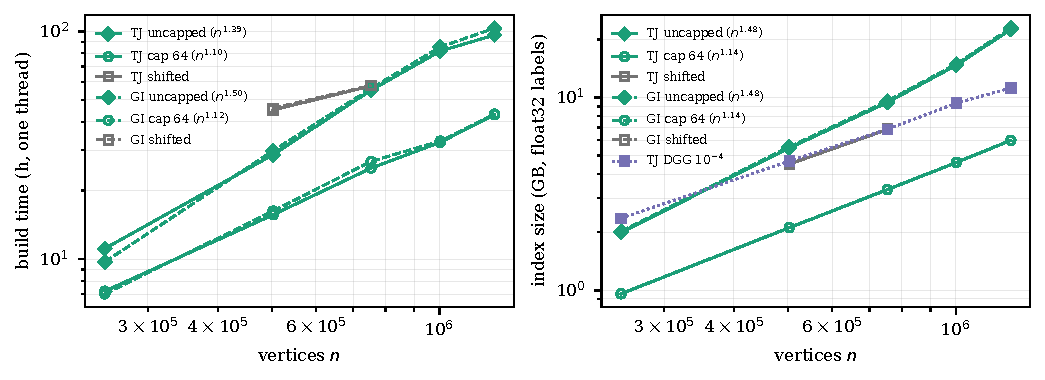
\includegraphics[width=0.92\textwidth]{figures/fig_scaling.pdf}
\caption{Build time and index size from 0.5M to 2.5M faces on TJ and GI, with the exponents of a power-law fit, and
DGG's graph for comparison.}
\label{fig:scaling}
\end{figure*}

\paragraph{Scaling to 2.5M faces.}
Table~\ref{tab:scale} and Figure~\ref{fig:scaling} follow TJ and GI from 0.5M to 2.5M faces (1.25M vertices).
The uncapped index stores labels growing like $n^{1.50}$, exactly the $\Theta(n^{1.5})$ of
Table~\ref{tab:complexity}, and reaches 23\,GB (15\,GB with 8-bit codes) at 1.25M vertices; its build grows like
$n^{1.4}$--$n^{1.5}$ and takes 96--103\,h on one thread. With cap 64 the labels grow like $n^{1.15}$, the index takes
6.0\,GB (2.1\,GB with 8-bit codes) at 1.25M vertices, and the build takes 43\,h. The query time stays at
0.33--0.38\,$\mu$s capped and grows from 1.1 to 2.7\,$\mu$s uncapped, while the mean error does not grow: it falls
from 0.0012\% to 0.0006\% uncapped and stays at 0.019--0.027\% capped. All answers at every size are certified and
correct. The parallel build on the 2.5M-face TJ takes 15.0, 10.3 and 9.6\,h with 8, 16 and 32 threads, against
96.3\,h on one, with labels bit-identical to the single-threaded build; the speed-up flattens beyond 16 threads,
where the top cuts, whose sweeps run on large sub-meshes, dominate. The shifted hierarchy, 1.4 times larger than the kd
hierarchy at 100k vertices, is smaller from 1M faces on (4.5 against 5.5\,GB at 1M, 6.8 against 9.4\,GB at 1.5M),
the crossover its constants predict, but its mean error is 0.08--0.09\% and it builds more slowly, so cap 64
(2.1 and 3.3\,GB at 0.02\%) dominates it. DGG's graph grows linearly and is smaller than our uncapped index from 1M faces, but larger than
the capped one at every size, and its queries slow down from 0.8 to 3.7\,s. From its memory growth EAR-Oracle would need about
0.9\,TB at 1M faces, more than the 768\,GB of a node.

\paragraph{Ablations.}
On TJ and GI at 0.5M faces the cap trades size for error smoothly: caps of 8, 16, 32, 64, 128 and 256 portals give
413\,MB to 1.70\,GB (float32), with mean errors from 0.55--0.64\% down to 0.002\%, and the exact refine is needed for
128--137 of the 2,000 random pairs with cap 8 and for none from cap 128. Thorup-style $\eps_c$-covers are dominated:
with $\eps_c=0.05$ they take 483\,MB for a mean error of 0.82\%, worse than cap 8 at 413\,MB, and with
$\eps_c=0.01$ 1.13\,GB for 0.082\%, against 0.0017\% for the uncapped 8-bit index at 1.02\,GB. For the label
sweeps, MMP alone takes 17--19\,h with 3\,GB of memory, VTP alone 11\,h with 199\,GB, and the hybrid 10\,h with
17\,GB, or 9\,h with 41\,GB when it prefers VTP more often.

\begin{table*}[t]
\caption{Obstacles on TJ and GI at 0.5M faces (disks covering 5, 10 and 20\% of the area, and six walls with gaps),
vertex pairs. Ours: $\eps=0.2$, $g=1$, float32. The detour column counts the random pairs whose distance is at least
1.2 times the straight-line distance, with our mean error on them. Every answer of ours is certified and correct.
EAR-Oracle: 5 Steiner points (the TJ walls run used 7); its other obstacle runs are still in progress.}
\label{tab:server-obst}
\small
\begin{tabular}{@{}ll|rrrr|rr|r|rr|rr@{}}
\toprule
 & & \multicolumn{4}{c|}{ours, uncapped} & \multicolumn{2}{c|}{ours, cap 64} & DGG $10^{-3}$ & \multicolumn{2}{c|}{NeuroGF} & \multicolumn{2}{c}{EAR-Oracle}\\
 & obstacles & size & mean & max $\UB$ & detour $\ge 1.2$ & mean & max $\UB$ & mean & mean & max & mean & max\\
\midrule
\multirow{4}{*}{TJ} & disks 5\% & 1.77\,GB & 0.0018\% & 1.92\% & 11, 0.0032\% & 0.016\% & 4.64\% & 0.034\% & 0.49\% & 9.8\% & -- & --\\
 & disks 10\% & 1.53\,GB & 0.0021\% & 0.57\% & 17, 0.0056\% & 0.021\% & 1.97\% & 0.036\% & 0.49\% & 8.1\% & 2.72\% & 9.65\%\\
 & disks 20\% & 1.33\,GB & 0.0022\% & 0.19\% & 41, 0.0082\% & 0.018\% & 2.43\% & 0.033\% & 0.50\% & 20.4\% & -- & --\\
 & six walls & 1.92\,GB & 0.0031\% & 0.79\% & 265, 0.0047\% & 0.032\% & 2.76\% & 0.035\% & 0.44\% & 12.4\% & 2.02\% & 6.63\%\\
\midrule
\multirow{4}{*}{GI} & disks 5\% & 1.80\,GB & 0.0021\% & 1.93\% & 4, 0.0099\% & 0.023\% & 5.63\% & 0.033\% & 0.50\% & 19.9\% & -- & --\\
 & disks 10\% & 1.54\,GB & 0.0022\% & 1.21\% & 21, 0.0025\% & 0.023\% & 3.07\% & 0.034\% & 0.51\% & 8.3\% & 2.93\% & 8.81\%\\
 & disks 20\% & 1.34\,GB & 0.0023\% & 1.00\% & 50, 0.0049\% & 0.020\% & 1.33\% & 0.032\% & 0.53\% & 23.4\% & -- & --\\
 & six walls & 1.95\,GB & 0.0048\% & 0.74\% & 285, 0.0165\% & 0.038\% & 1.50\% & 0.033\% & 0.50\% & 15.9\% & -- & --\\
\bottomrule
\end{tabular}
\end{table*}

\paragraph{Obstacles.}
Table~\ref{tab:server-obst} repeats the obstacle experiment at 0.5M faces. Our mean error is 0.002--0.005\%
uncapped and 0.016--0.038\% capped, as without obstacles, and stays that low on the pairs whose path has to go around
the obstacles: on the walls meshes 265 and 285 of the 2,000 random pairs have a detour of at least 20\%, with mean
errors of 0.005\% and 0.017\%. Every answer is certified and correct. The walls make the build about twice as
long (22--25\,h uncapped), because detours widen the windows. DGG keeps its accuracy (0.03\%) at 0.2\,s per query,
EAR-Oracle keeps its 2--3\%, and NeuroGF's maximum error grows to 16--23\% on some meshes. The two exact
solvers disagree at a few vertices, on these meshes mostly at hole boundaries and occasionally also inside plain
terrains: VTP returns distances that are too long, by up to 1.3\% here and up to 3\% at rare vertices of the 1M-face
TJ, which we confirmed with Steiner paths shorter than VTP's value, while MMP, our ground truth, is never above such a
path. Our hybrid build uses VTP for some sweeps, so a few labels can be too long. That keeps every
$\UB$ an upper bound but could in principle push a $\LB$ above the true distance; it did not happen on any of the
checked pairs, and a build with MMP alone avoids it.

\paragraph{kNN and range queries in the POI setting.}
UP-Oracle's own workload asks for distances between points of interest, and we ran kNN ($k=1,10,25$) and range
queries (radius 1, 3 and 10\% of the chart diagonal) from 20 of them over all others, with their POI files of 50,
500 and 2,500 points on the six terrains at 0.5M faces. The UP-Oracle family has no proximity operator, so it
answers every query-object pair. Our index over the POIs takes 1.2, 2.4--2.6 and 6.7--7.3\,MB and builds in
4--5\,h. Its certified-approximate kNN with $k=10$ takes 29--73\,$\mu$s with recall at least 99.5\%, and range
queries 2--93\,$\mu$s. UP-Oracle takes 0.7--0.8\,ms per kNN query with 50 POIs, 50--72\,ms with 500 and 97--122\,s
with 2,500, where its index is 2.1--2.4\,GB and builds in 19--25\,h; WSPD-Oracle and RC-Oracle are faster at 2,500
POIs (2.6--5.9\,s) but slower at 50 and 500. DGG with an early-stopping Dijkstra takes 20--26\,ms at 50 POIs and
0.14--0.20\,ms at 2,500. Our exact mode needs sweeps when the POIs are sparse: 0.1--0.9\,s at 50 POIs,
0.7--8.9\,ms at 500 and 0.06--0.5\,ms at 2,500. In the plain POI setting, distances between POIs only, our POI index
answers in 0.7--0.9\,$\mu$s with a mean error of 0.003--0.008\%, against UP-Oracle's 0.4--2.3\% at 15\,$\mu$s to
57\,ms; but the exact $P\times P$ table built with one VTP sweep per POI stays the best choice up to 2,500 POIs
(25\,MB, 0.04--3\,h), as on the small terrains.

\paragraph{Proximity over many objects.}
With 10,000 random objects at 0.5M faces, certified-approximate kNN answers in 33--130\,$\mu$s for $k=1$ and
54--154\,$\mu$s for $k=10$ with recall of at least 98.9\%. The exact mode needs a sweep only for the candidates near
the answer boundary: 38--140\,$\mu$s for $k=1$ and 0.3--0.4\,ms for $k=10$, against 2.7--3.2\,s for one exact
sweep from the query point. At 2.5M faces, $k=10$ takes 0.6\,ms approximately and 2.6\,ms exactly, against an 11\,s
sweep.

\paragraph{The small terrains on the cluster.}
Rerunning the small-terrain configurations of Table~\ref{tab:main} on the cluster gives the same picture: on
Gunnison10k with $\eps=0.1$ the build takes 194\,s (202\,s on the laptop) and the mean error is 0.0076\%.

\section{Discussion}
\label{sec:discussion}

The experiments support the main claim: a terrain distance oracle can answer in about a microsecond and
certify every answer, with errors far below those of the Steiner-graph oracles and an index two to three orders
of magnitude smaller, up to terrains with millions of faces. The certificate is what makes the index usable as a database operator. A kNN or range query can
decide most candidates from the intervals alone, and a user who needs a guaranteed answer can ask for $\UB$, which is
the length of an actual path, or for an exact refinement only when the interval is too wide. DGG reaches a similar
accuracy with a much shorter build, and the two are complementary: DGG is a compact surface model searched per query,
our index precomputes the answers, which pays off after a few thousand to a few tens of thousands of queries.

\subsection{Limitations}

\paragraph{Asymptotic size.}
The uncapped index stores $\Theta(n^{1.5})$ labels, as the top cuts have $\Theta(\sqrt n)$ portals and every vertex
stores them. The capped variant is near-linear, but its $(1+\eps)$ guarantee relies on the exact refine for the rare
close pairs across a capped cut, and Djidjev and Sommer's oracle is asymptotically smaller in theory.

\paragraph{Build.}
The build is dominated by one exact sweep per portal. Uncapped it grows like $n^{1.4}$--$n^{1.5}$ and takes 96\,h
on one thread at 2.5M faces (9.6\,h on 32 threads), and capped 43\,h; DGG builds its graph in minutes. The build is
the price of the certificate and of microsecond queries, and it is recovered after roughly 6,000--50,000 queries,
depending on the variant and the alternative.

\paragraph{Slopes and weights.}
$\lambda$ enters the near radius, the window and the ellipse. Steep terrains do not change $\lambda$, but heavily
weighted terrains with a small $w_{\min}$ widen all three, and on weighted terrains the labels are Steiner distances,
so we certify only the upper bound.

\paragraph{Static terrains.}
The index is static. Terrains that change, the setting of UP-Oracle, would need the affected cuts rebuilt.

\section{Conclusion}

We introduced the Certified Cut Index, a distance oracle for terrain surfaces that stores exact geodesic distances
to portals sampled on the cut lines of a kd hierarchy and returns every distance with a certified interval within a
factor $1\pm\eps$. The window lemma lets the cuts be sampled, the ellipse lemma makes the labels exact and cheap to
compute, and the 1-Lipschitz label rows give the lower bound. The index answers in a fraction of a microsecond,
is far more accurate and smaller than the existing terrain oracles, and extends to arbitrary points, proximity
queries, weighted terrains and obstacles, and scales to terrains with millions of faces. Future work includes a
faster build, updates for changing terrains, and closing the gap to near-linear space without the refine step.

\section*{AI use statement}
We used generative AI tools to help write and test parts of the implementation and the experiment scripts, to
summarise related literature, and to draft and edit parts of this manuscript. The author reviewed the code, checked
the cited works against the original sources and verified the proofs and the experimental results, and takes full
responsibility for the content.

\bibliographystyle{ACM-Reference-Format}
\bibliography{refs}

\appendix

\section{Proofs}
\label{app:proofs}

We use the notation of Section~\ref{sec:index}. In the implementation a portal that falls within $10^{-7}$ of a face
edge is moved along the line by about $10^{-5}$ edge lengths before it is inserted, so a run end may not be a portal.
It then leaves an end stretch $[\text{run end},p_k]$ of arc $e_k$, and the lower bound also takes the term $f_k-2e_k$.

\begin{lemma}[crossing]
Every curve on $T$ between two points on opposite sides of $\ell_C$ meets $\ell_C$.
\end{lemma}
\begin{proof}
The $a$-coordinate of its chart projection is continuous, below $v$ at one end and above at the other.
\end{proof}

\begin{proof}[Proof of Lemma~\ref{lem:sandwich} with end stretches]
If the crossing $x^\ast$ lies in an end stretch with portal $p_k$, then $f_k\le d(s,x^\ast)+2A(x^\ast,p_k)+d(x^\ast,t)
\le d(s,t)+2e_k$, so $f_k-2e_k\le d(s,t)$. The interval case is as in the main text.
\end{proof}

\begin{proof}[Proof of Theorem~\ref{thm:main}]
Let $|s-t|>R$ and $d=d(s,t)$, so $d\ge\lambda|s-t|>g/\eps$ by~\eqref{eq:lower}. Let $x^\ast$ be the crossing of a
shortest path in the interval $[p_j,p_{j+1}]$ with arc gap $A_j$, and $a=A(p_j,x^\ast)$.

\emph{Upper bound.} $\min(f_j,f_{j+1})\le d+\min(2a,2(A_j-a))\le d+A_j$. If the interval lies in $I_C$ then
$A_j\le g<\eps d$. Otherwise every point of the interval, $x^\ast$ included, has offset at least $c_j$ from $I_C$, so
$d\ge 2\lambda c_j$ by Lemma~\ref{lem:window}, and~\eqref{eq:gaps} gives $A_j\le\max(g,2\eps\lambda c_j)\le\eps d$. In
an end stretch, $f_k\le d+2e_k$, and $2e_k$ is far below $g<\eps d$.

\emph{Lower bound.} Every $f\ge d$, so an interval term satisfies $\frac12(f_j+f_{j+1})-A_j\ge d-A_j$, which is at
least $(1-\eps)d$ if $A_j\le\eps d$. Otherwise $A_j>\eps d>g$, so the interval is a tail interval with
$A_j\le 2\eps\lambda c_j$, hence $c_j>d/(2\lambda)$. Both of its portals $p$ have offset at least $c_j$ from $B_M$,
so by~\eqref{eq:lower} $f(p)\ge\lambda(|s-p|+|p-t|)\ge 2\lambda c_j$, and the term is at least
$2\lambda c_j(1-\eps)>(1-\eps)d$. An end-stretch term is $f_k-2e_k\ge d-2e_k>(1-\eps)d$. The chord term is a lower
bound, so $\LB\ge(1-\eps)d$.
\end{proof}

\begin{proof}[Proof of Theorem~\ref{thm:capped}]
Lemma~\ref{lem:sandwich} holds for any portal set, so $\LB\le d\le\UB$. The proof of Theorem~\ref{thm:main} used
$g<\eps d$ only through the gap inside $I_C$; with gap $g_C$ it gives $\UB\le(1+\eps)d$ whenever $g_C\le\eps d$, and
the query refines every pair for which this is not certified, that is every pair with $\UB>(1+\eps)\LB$. A refined
pair is computed by one exact sweep on the faces meeting $\mathrm{bbox}(s,t)$ dilated by $\UB/(2\lambda)$, which
contains every path of length at most $\UB$ by Lemma~\ref{lem:ellipse}, so it is exact.

For the size, a cut has at most $k$ portals in its box. In a tail the gap is $g_C$ until $2\eps\lambda c\ge g_C$,
which takes $O(g_C/(2\eps\lambda)/g_C)=O(1/\eps)$ portals, and from then on the offset grows by a factor at least
$1+2\eps\lambda/\sigma$ per portal, up to the window length $\mu_C/\lambda$. With $\mu_C\approx D_C$ and
$g_C\approx\sigma D_C/k$ for a cut of length $D_C$, this takes $O\big(\frac{\sigma}{\eps\lambda}\log\frac{2\eps k}{\sigma}\big)
=O(\eps^{-1}\log k)$ portals. A vertex lies in $O(\log n)$ cuts, which gives the label count.
\end{proof}

\begin{proof}[Proof of Theorem~\ref{thm:a2a}]
$\UB(p,q)$ is the cost of a path from $p$ to a corner, then a path certified by $\UB(a_i,b_j)$, then to $q$. For the
lower bound, $d(a_i,b_j)\le d(a_i,p)+d(p,q)+d(q,b_j)\le w_f|P-A_i|+d(p,q)+w_{f'}|Q-B_j|$, so every term of the
maximum is at most $d(p,q)$. Pairs whose interval is wider than $1+2\eps$, and near pairs, are computed exactly on an
ellipse sub-mesh with both points inserted as vertices.
\end{proof}

\end{document}
